\documentclass[a4paper]{IEEEtran}
 
\usepackage{amsmath}
\usepackage{graphicx}
\usepackage{caption}
\usepackage{subfigure}
\usepackage{epstopdf}
\usepackage[ansinew]{inputenc}
\usepackage{listings}
\usepackage{xcolor}
%\setlength{\oddsidemargin}{0cm}
%\setlength{\evensidemargin}{0cm}
%\setlength{\topmargin}{0cm}

\usepackage[]{algorithm2e}

\usepackage{a4wide}

\title{ Allen mouse brain circuit building validation}
%\author{Till Schumann, Fabien Delalondre}
%\date{}

\begin{document}
   \maketitle
   
   \section{Description}
   A simulation of a full scale point neuron circuit of the mouse brain make great demands on the simulator, circuit generation and the used data formats.   
   
   The full point neuron circuit contains about $75e6$ neurons with $1e4$ synapses per neuron.
   To make such a large scale simulation possible with NEST software, we had to adapt the NEST model building process to be able to consume
experimental data. This adaptation required providing a new implementation of the NEST C++ "import functionality" so that it can load a data-driven circuit from HDF5 files (around $10$ TB) efficiently. The current implementation has been made functional on IBM Blue Gene/Q up to 2 racks (2048 nodes).   

The used HDF5 file which contains the long range connection information has been generated by analyzing injection experiment data provided by the 
Allen Brain Institute which provides a high-resolution map of neural connections in the mouse brain.
The experiment datasets contain a 3D volumetric data of the injection and a 3D volumetric data of its axonal projection labeled by viral
   tracers. Connections are created from neurons inside the injected regions to neurons inside the projected regions.
  
	 \begin{figure}[ht!]
   	\begin{center}
        \subfigure[Injection sites - showing all available experiments]{%
            \label{fig:allInjections}
            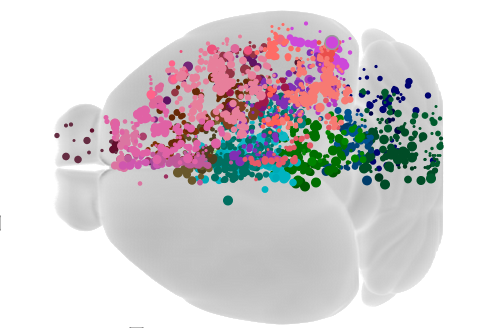
\includegraphics[width=0.24\textwidth]{../connectionBrowser_allinjections.png}
        }
        \hspace{0.1cm}
        \subfigure[Projection of one experiment]{%
            \label{fig:oneProjection}
            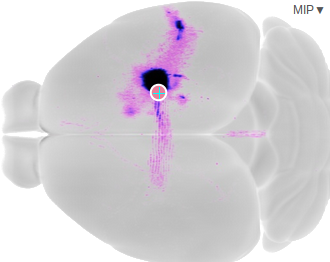
\includegraphics[width=0.19\textwidth]{../connectionBrowser_oneinjections.png}
       }
    	   \end{center}
    	\caption{%
        The pictures are inverted and copied from the Allen Brain Atlas.
     }%
   \label{fig:atlas}
   \end{figure}  
  
   
   %To import the circuit into NEST, we implemented a module that allows the loading of the synapse information and circuit topological information from the hdf5 file.
   In order to validate the built model, we wish to proceed in the following two steps
\begin{itemize} 
\item We first would like to validate topologically the built model by comparing images provided by the Allen Institute of Injection experiment against 
similar images built from numerical modeling. To this end, we wish to build visual representation of the projection data and do a direct pixel comparison between images. The bulk of the work will then consist of building a metric similar to the injection metric and provide comparison metric/methods between two images.
\item After the first validation would be passed, we wish to observe the spiking activity of the resulting model and ensure that all spikes generated are only transmitted via the expected long range connections. 
\end{itemize}
   
   \section{Given data}
   \begin{itemize}
      \item x,y,z coordinates of neurons in hdf5 file
      \item synapses (source and target neuron ids) in hdf5 file
	  \item 3D volumetric injection and projection densities with $100\mu m$ voxel resolution in NRRD format
	  (http://help.brain-map.org/display/mouseconnectivity/API\#API-3DReferenceModels)
	  \item 3d volumetric number of neurons per voxel with $100\mu m$ resolution (C style, int values)
   \end{itemize}
   
   \begin{figure}[ht!]
   	\begin{center}
        \subfigure[Number of excitatory neurons per voxel. The plot (x vertical and z horizontal axis) show a slice (along the y axis) of the 3D datasets.]{%
            \label{fig:allInjections}
            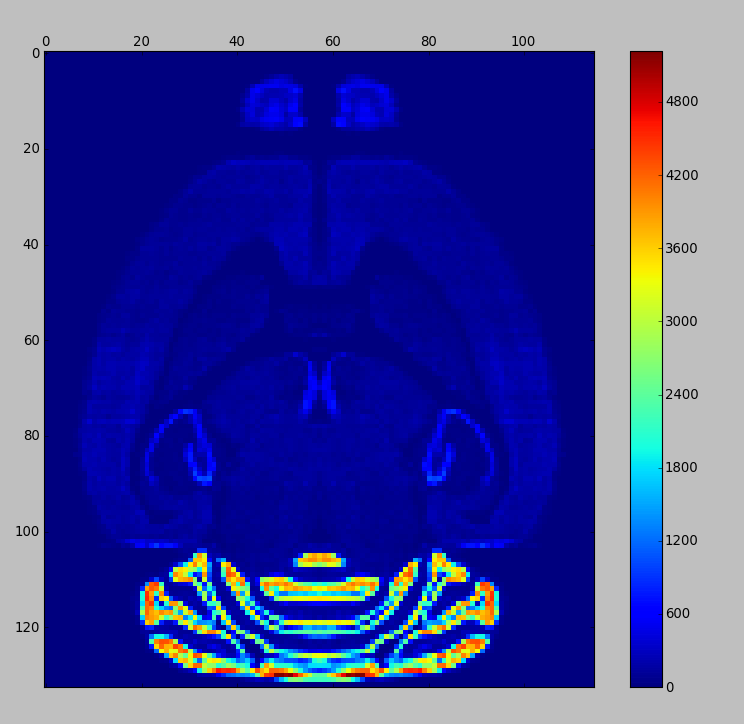
\includegraphics[width=0.2\textwidth]{../exNeurons_numPerVoxel.png}
        }
        \hspace{0.1cm}
        \subfigure[Illustration of neurons inside an injection and projection area]{%
            \label{fig:oneProjection}
            \includegraphics[width=0.18\textwidth]{drawing.eps}
       }
    	   \end{center}
    	%\caption{% 
    % }%
   \label{fig:atlas}
   \end{figure}
   
\end{document}
